\classheader{2018-06-19}
\subsection*{Modeling with First Order Equations}
This section deals with applications and the details of how to model a process to construct on ODE.\\
This, in general, is a difficult process and quite \underline{ad hoc}. Also it cannot be mastered in such a short time. Read this section.\\
\redhline\\
\subsection*{Non-Linear Equations}
In all examples shown, there has always been a solution. And with initial data, there has always been an \underline{unique solution.}
Is this always the case?\\
\begin{example-N}
	Solve $(y')^2 + 1 = 0$\\
	(Find a function whose derivative is -1?)
\end{example-N}
\begin{example-N}
	Solve $y' = \frac{3}{2} y^{\frac{1}{3}}$, $y(0)=0$\\
	Note that here that \circled{a} $y(t) \equiv 0$ solves this. But so does \circled{b} $y(t) = t^{\frac{3}{2}}$ \quad  \circled{c} $y(t) = -t^{\frac{3}{2}}$
	\begin{center}
	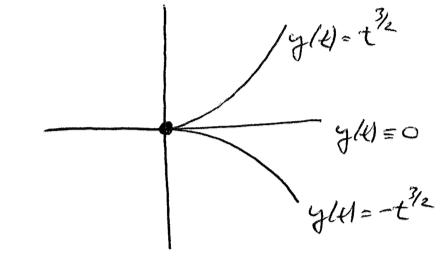
\includegraphics{5-1}		
	\end{center}

	Since all three of those distinct functions solve the IVP, we say solutions here (at $y(0)=0$) are \underline{NOT unique}!\\
\end{example-N}
\textbf{Question: } 16 Solutions to an ODE are not unique at a point $y(t_0) = y_0$, then 2 or more solutions that are distinct pass through the point. What does this say about the predictive power of your model?
\begin{center}
	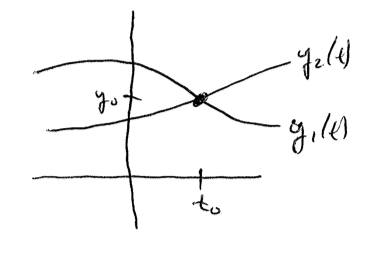
\includegraphics{5-2}
\end{center}
There are criteria for ensuring an IVP has solutions (sols. exist) and whether they are unique or not (unique is good!)\\\\
Let $(\star)\quad  y'(t) = f(t,y)$, $y(t_0) = y_0$ be an IVP
\begin{theorem-N}
	If $f(t,y)$ and $\dfrac{df}{dy}(t,y)$ are continuous in some rectangle $\alpha < t < \beta, \gamma < y < \delta$ containing $(t_0, y_0)$, then in some interval $t_0 - h < t < t_0 + h$ inside $\alpha < t < \beta$, there exists a unique solution $y(t)$ to $(\star)$\\
\end{theorem-N}

{\Large \underline{Many comments}}
\begin{enumerate}[label=\protect\circled{\alph*}]
	\item $f(t,y)$ and $\dfrac{df}{dy}(t,y)$ are functions of 2 variables. Continuity here is bigger than simply continuous in each variable while holding the other variable constant.
	\item $\dfrac{df}{dy}(t,y)$ is the derivative of $f$ with respect to $y$ while pretending $t$ is a constant.. It is called a \underline{partial derivative}.
	\item Geometrically, a solution passing though $(t_0, y_0)$ is an integral curve in the $ty-plane$.\\
	\begin{center}
		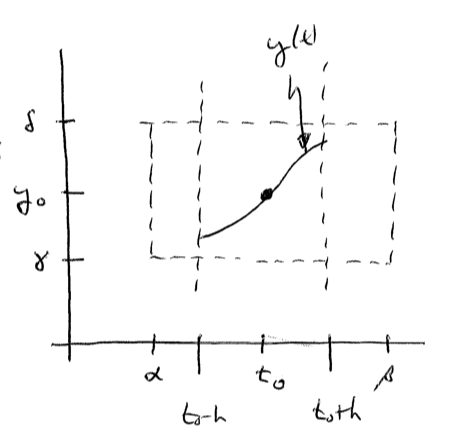
\includegraphics[scale=0.7]{5-3}		
	\end{center}
	\item $f(t,y)$ is continuous near $(t_0, y_0)$, then $y'(t)$ is continuous. But then by Calc I, $y(t)$ is differentiable. Hence solution \underline{exists} through $(t_0, y_0)$\\
	By Fundamental Theorem of Calculus, $y(t) = y(t_0) + \int_{t_0}^t f(s, y(s)) ds $.\\
	Since  $f(t,y)$ is continuous near $(t_0, y_0)$, then this integral will \underline{exist}. Note:
	\begin{equation*}
		y' = \dfrac{d}{dt}\bigg[y(t)\bigg] = \dfrac{d}{dt}\bigg[\int_{t_0}^t f(s, y(s)) ds\bigg] = f(t,y)
	\end{equation*}
	\item if $\dfrac{df}{dy}(t, y)$ is continuous near $(t_0, y_0)$, then solutions very nicely in the y-direction. This is enough to ensure solutions are \underline{unique}.\\
	$\Rightarrow$ Solution curves never touch or cross when uniquely defined. 
	\item \underline{Example: } Given $ty' + 2y = 4t^2$, if we place it in the form $y' = f(t,y)$, we set $y' = -\frac{2}{t}y + 4t$\\
	Here, as long as our initial data does not include $t_0 = 0$, solutions will exist\\ ($-\frac{2}{t}y + 4t$ is cont when $t\neq 0$) and unique when ($\dfrac{df}{dy}(t,y) = -\frac{2}{t}$ is continuous when $t \neq 0$)\\
	\textbf{Caution: } it may be possible for solutions to exist and/or be unique when $t=0$. But it is not assured!
	\begin{example-N}
		Given $y' = \frac{3}{2} y^{\frac{1}{3}}$, $f(t,y) = \frac{3}{2} y^{\frac{1}{3}}$.\\
		Here $f(t,y)$ is defined and continuous everywhere (and for all $t\in \mathbb{R}$, and $y \in \mathbb{R}$). Hence by Thm, \underline{solutions} are guaranteed to exist everywhere.\\
		But $\dfrac{df}{dy}(t,y) = \frac{1}{2}y^{-\frac{2}{3}}$ is not continuous along the $y=0$ line (in the $ty-plane$). Hence solutions exist for starting values like $y(t_0) = 0$, but \underline{may not be unique} (everywhere else they are unique!)
	\end{example-N}
	For any value $c \geq 0$, the curve $y(t) = 0, (t < c)$ and $(t-c)^{\frac{3}{2}} when, (t \geq c)$.\\
	Solve the IVP $y' = \frac{3}{2}y^{\frac{1}{3}}$, $y(0) = 0$
	\begin{center}
		\begin{tikzpicture}
			\begin{axis}
			[ymin = -1, ymax = 2,
			xmin = -1, xmax = 5,
			axis lines=center,
			axis on top=true,
			domain=0:4,
			xlabel={$x$},
    		ylabel={$y$},
    		samples=100]
    		\addplot[mark=none, draw=black, thin]{(x-0)^(3/2)} node [pos=0, below right, color=red]{$c=0$};
    		\addplot[mark=none, draw=black, thin]{(x-1)^(3/2)} node [pos=0, below right, color=red]{$c=1$};
    		\addplot[mark=none, draw=black, thin]{(x-2)^(3/2)} node [pos=0, below right, color=red]{$c=2$};
			\end{axis}
		\end{tikzpicture}
	\end{center}
	\item For linear ODE, existence and uniqueness is easier. In standard form,
	\begin{equation*}
		y' + p(t)y = q(t)
	\end{equation*}
	\begin{center}
		and in $y' = f(t,y)$ form
	\end{center}
	\begin{equation*}
		y' = \underbrace{-p(t)y + q(t)}_{f(t,y)}
	\end{equation*}
	\begin{theorem-N}
		As long as $p(t)$ and $q(t)$ are continuous at $t_0$, then solutions exist and are unique for $y' = -p(t)y + q(t)$, $y(t_0) = y_0$
	\end{theorem-N}
\end{enumerate}